\documentclass[10pt,a4paper,oneside]{scrartcl}

%\usepackage[ngerman]{babel}   % Deutsches Proposal
\usepackage[USenglish]{babel} % English proposal

\usepackage[utf8]{inputenc}
\usepackage{hyperref,xcolor,microtype,ifthen}

\setkomafont{disposition}{}
\setkomafont{descriptionlabel}{\bfseries}

\usepackage[textwidth=450pt]{geometry}

\usepackage[backend=bibtex,style=ieee,hyperref,natbib]{biblatex}

\usepackage{graphicx}
\graphicspath{{./res/}}

\usepackage{pgf-umlcd}

\usepackage[]{algorithm2e}

\addbibresource{references.bib}

\usepackage{tikz}
\usetikzlibrary{shapes,arrows}
% Kommentare abschalten
% Disable the hints here
\newboolean{showhints}
\setboolean{showhints}{true}
%\setboolean{showhints}{false}

\newcommand\hint[2]{
	\ifthenelse{\boolean{showhints}}{
		\begin{center}
			\colorbox{black!10}{
				\begin{minipage}{.963\textwidth}
					#2\hfill\textbf{#1}
				\end{minipage}
	}\end{center}}{}
}

%Title of the proposal
\title{Automatic Change Recommendation using Decision Trees}
%bachelor or master?
\subtitle{Bachelor Thesis Proposal}
%first and then last name
\author{Valentin Reyes Häusler}

\begin{document}
	
	\maketitle
	
	\section{\iflanguage{ngerman}{Einführung und Motivation}{Introduction and Motivation}}
	\label{sec:motivation}
	
	- Design phase is a core step in any software development process
	\\
	- Objective of design phase: creation of design for architecture, software components, interfaces and data (IEEE-Standard "design phase")
	\\
	- This is accomplished by creating models and meta-models describing the solution precisely and completely while maintaining a necessary level of abstraction. (Skript 07.1)
	\\
	- For example: In object-oriented modeling class diagrams are indispensable. \ref{classDiag} shows classes and their relationships such as dependencies and associations. 
	\\
	- Importance of models: 
	Recognition of patterns and redundancies allowing simplification (creation of a super class) 
	... (TODO: more examples)
	\\
	- It is clear that a precise and complete design serves as a stable base for an efficient implementation.
	\\
	- Tools for the latter phase are vastly available. They range from code completion and action recommendation to generation of complete blocks of code.
	\\
	- This allows the engineer to concentrate on the core tasks of the implementation phase.
	\\
	- Although the design phase is equally important, comparable tools are often lacking or non existent.
	\\
	- A possible improvement in this aspect are automatic action proposals for the creation of models.
	\\
	- Basic to semi-complex actions such as the creation of a super class, separation of packages and so on, could be proposed to the designer.
	\\
	- Such a tool would again allow the engineer to concentrate on the core tasks of a consistent and complete design.
	\\
	- This thesis aims to create and evaluate such a tool.
	\\
	- We intend to do this by analyzing the versionized histories of models
	\\
	- Using machine learning algorithms and data structures we look for reoccurring patterns
	\\
	- The patterns are then matched to a model which is being worked on. 
	\\
	- If a fit is found a recommendation can be done.
	\\
	- Example for class diagrams:\\
	Pattern:
	State: Two classes X and Y share some attributes and functions\\
	Actions: \\
	\begin{itemize}
		\item Create superclass Z for X and Y
		\item Move shared attributes and functions from Y to Z
		\item Delete the same attributes and functions from X
	\end{itemize}
	Abstraction: Pull up shared attributes/functions to superclass
	\begin{center}
		\begin{figure}
			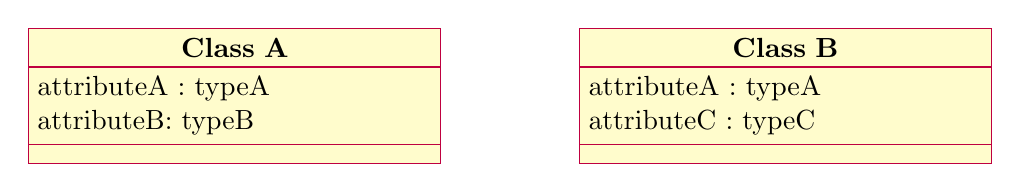
\begin{tikzpicture}
			\begin{class}{Class A}{0,0}
			\attribute{attributeA : typeA}
			\attribute{attributeB: typeB}
			\end{class}
			
			\begin{class}{Class B}{7,0}
			\attribute{attributeA : typeA}
			\attribute{attributeC : typeC}
			\end{class}
			\end{tikzpicture}
			\caption{Class diagram. Class A and class B share attributeA.}
		\end{figure}
	\end{center}
	
	\begin{center}
		\begin{figure}
			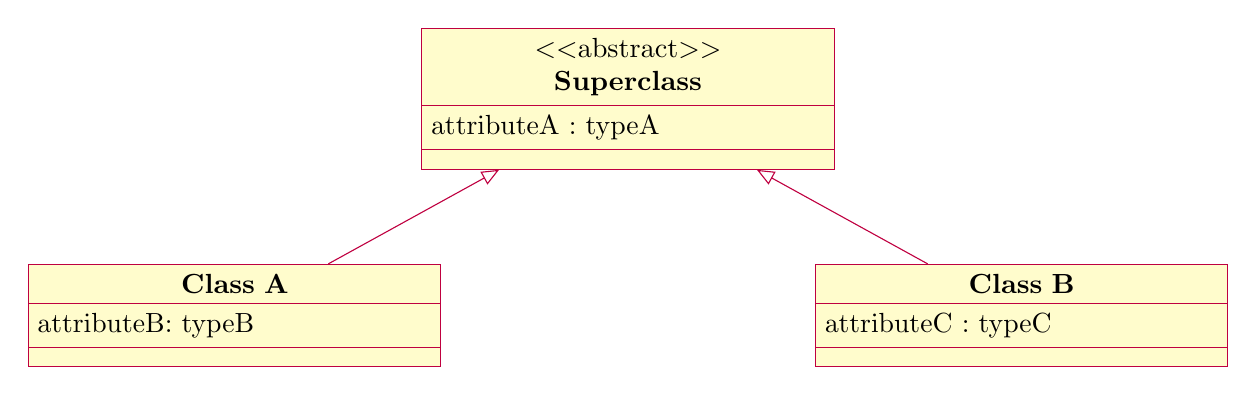
\begin{tikzpicture}
			\begin{abstractclass}{Superclass}{0,0}
			\attribute{attributeA : typeA}
			\end{abstractclass}
			
			\begin{class}{Class A}{-5,-3}
			\inherit{Superclass}
			\attribute{attributeB: typeB}
			\end{class}
			
			\begin{class}{Class B}{5,-3}
			\inherit{Superclass}
			\attribute{attributeC : typeC}
			\end{class}
			\end{tikzpicture}
			\caption{attributeA is "pulled up" from class A and B to Superclass. }
		\end{figure}
	\end{center}
	\section{\iflanguage{ngerman}
		{Problemstellung}
		{Problem Statement}}
	\label{sec:problem_statement}
	\begin{figure}
		\centering
		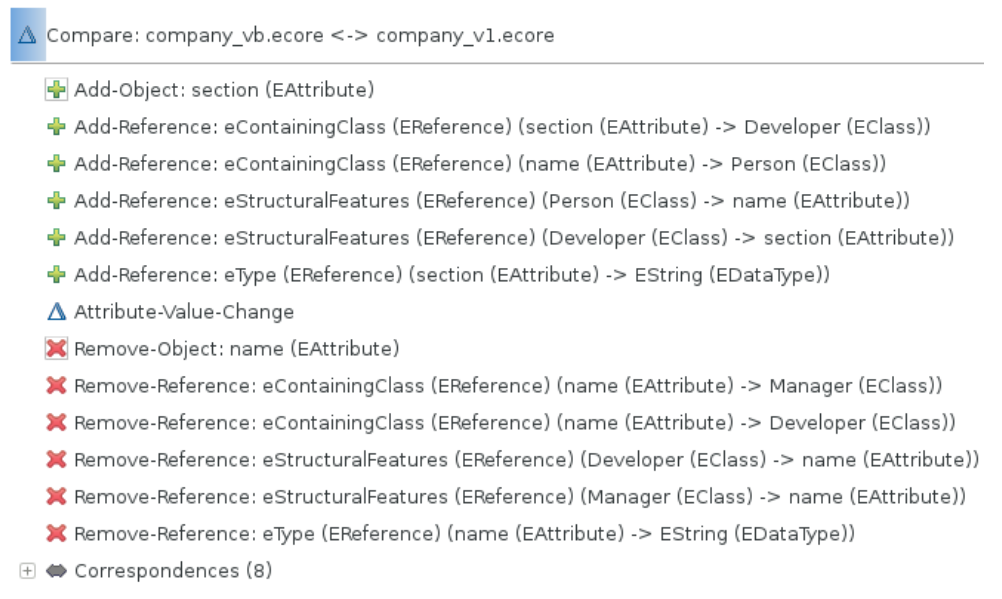
\includegraphics[width=0.9\textwidth]{./res/low-level-actions.png}
		\caption{Low-level differences between two models as recognized by SiLift}
		\label{fig:SiLiftEx}
	\end{figure}
	- SiLift is able to compare different versions of a model
	\\
	- It recognizes \textit{low-level} actions and dependencies between those actions.
	\\
	- Low-level actions are simple internal operations for the deletion and creation of objects and their references.
	\\
	- Figure \ref{fig:SiLiftEx} shows the low-level differences between two versions of the model \textit{company}.
	\\
	- User-level actions consist of various low-level actions.
	\\
	- For example: Creating a new string-attribute \textit{section} in the class \textit{Developer} consists of the low-level actions:
	\\
	\begin{enumerate}
		\item Create attribute: section
		\item Add containingClass-reference from section to Developer
		\item Add structuralFeatures-reference from Developer to section
		\item Add type-reference from section to String
		\item Change the value of section.
	\end{enumerate}
	- This example can be seen in \ref{fig:SiLiftEx}
	\\
	- Abstracting the individual actions we can create a \textit{recognition rule} for the user-level action INSERT \textless type\textgreater  \textless attr\textgreater=\textless val\textgreater  IN \textless class\textgreater :
	\begin{enumerate}
		\item Create attribute: \textless attr\textgreater
		\item Add containingClass-reference from \textless attr\textgreater  to \textless class\textgreater
		\item Add structuralFeatures-reference from \textless class\textgreater  to \textless attr\textgreater
		\item Add type-reference from \textless attr\textgreater  to \textless type\textgreater
		\item Change value of \textless attr\textgreater  to \textless val\textgreater
	\end{enumerate}
	- SiLift uses these recognition rules and \textit{lifts} matching sets of low-level actions to user-level actions.
	\\
	
	- We aim to automatically generate recognition rules from a model's history.
	\\
	- The initial data is given in from of a dependency graph.
	\\
	\begin{figure}
		\centering
		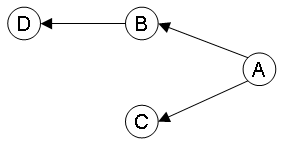
\includegraphics{./res/Dependencygraph.png}
		\caption{Dependency graph. A has to happen before B and C; B has to happen before D.}
		\label{fig:depgraph}
	\end{figure}
	- Nodes represent actions; edges dependencies.
	\\
	- Figure \ref{fig:depgraph} represents a dependency graph.
	\\
	- Note that since not every action has a dependency there can be multiple separated subgraphs and nodes without parents. 
	\\
	- We call this nodes orphan-nodes.
	\\
	- Generating the recognition rule for \textit{INSERT \textless type\textgreater \textless attr\textgreater=\textless val\textgreater IN \textless class\textgreater} we applied an abstraction to the low-level actions.
	\\
	-The abstraction consists of mapping the arguments of an action to variables.
	\\
	- For example: Create attribute: section becomes Create attribute: \textless attr0\textgreater with \textless attr0\textgreater = section.
	\\
	- With this abstraction two actions can be compared by simply comparing their abstracted version with one another.
	\\
	- When comparing action sequences checking whether the mapping and using of variables are consistent with each other.
	\\
	- If a variable is mapped to an object then all actions using that object must use the variable in the abstracted action sequence.
	\\
	- Now we are able to find recurring implementations of the same abstract user-level action.
	\\
	- We do this with following algorithm:
	\begin{algorithm}
		\KwIn{Dependency graph \textbf{G}}
		\KwOut{Decision trees for recommendation}
		\ForEach{Orphan Node \textbf{o}}{
			Create abstract version of action \textbf{a}\;
			Find tree \textbf{t} with \textbf{a} at it's root\;
			\If{No such tree exists}{Create one}
			With Breadth-First-Search:\\
			\ForEach{Path \textbf{p} reachable from \textbf{o} in \textbf{G}}{
				\If{\textbf{p} does not exist in \textbf{t} starting at the root}
				{Extend the longest matching path in \textbf{t} starting at the root to \textbf{p}\;}
				Reinforce the probability of the path in \textbf{t}\;
			}
			
		}
	\end{algorithm}
	- The construction of the data-structure automatically calculates the absolute number of occurrences of any path and with it the relative probability of it's occurrence.
	\\
	This allows us to match the last actions done by the user to the decision trees. 
	\\
	If a match is found the next nodes in the tree can be recommended according to their probability of occurrence.

	\textbf{TODO:} Example of bigger dependency graph and transformation to decision trees.

	
	\section{Purpose of the study}
	The purpose of this study is to create a tool for change proposal during the creation of models and meta models. Such a tool, if efficient, could provide support for engineers during the design phase of software comparable to autocompletion tools used during the implementation phase. 
	
	\section{\iflanguage{ngerman}
		{Verwandte Forschung}
		{Review of the literature}}
	
	Programming:\\
	Learning haskell data analysis\\
	Author: James Church\\
	Summary: The book gives an overview over the steps for data analysis. Practical examples with Haskell are given for every step.
	Significance: The methods for parsing and manipulating data taught in this book are applicable to the challenges of this thesis.\\
	
	
	Learn You a Haskell for Great Good!: A Beginner's Guide\\
	Author: Mirian Lipovaca\\
	Summary: Ample overview over Haskell's functionality.\\
	Significance: This book builds a stable base for learning Haskell.\\
	
	
	Foundation:\\
	Understanding Model Evolution through Semantically Lifting Model Differences with SiLift\\
	Authors: Timo Kehrer, Udo Kelter, Manuel Ohrndorf, Tim Sollbach
	Summary: This paper presents SiLift. SiLift is able to lift low-level differences of models into user-level actions.\\
	
	
	Automatic Change Recommendation of Models and Meta Models Based on Change Histories\\
	Authors: Stefan Kögel, Raffaela Groner, and Matthias Tichy\\
	Summary: Alternative aproach ... TODO\\
	Significance: The results presented in this paper are comparable to our results. It would be interesting to compare effectiveness of both tools.\\
	
	\section{\iflanguage{ngerman}
		{Forschungsfragen}
		{Research questions and/or Hypotheses}}
	\label{sub:questions}
	
	\begin{description}
		\item[RQ1:] How much data is necessesary for the tool to perform relatively well?
		\item[RQ2:] Are there cases in which the tool performs better or worse?
		\item[RQ3:] How does this tool compare to other implementations?
		\item[RQ4:] Is it possible to use this aproach for other applications?
		\item[RQ5:] If so, how has the data to be processed to the aproach to be applicable?
	\end{description}
	
	\section{\iflanguage{ngerman}
		{Eigener Ansatz}
		{The Design - Methods and Procedures}}
	\label{sec:approach}
	Hevner presented 7 guidelines for design science research:
	\begin{description}
		\item[Design as an artifact:] The aim of this paper is to produce an autorecommendation tool.
		\item [Problem relevance:] Comparable tools are often lacking or non-existent.
		\item [Design evaluation:] This tool will be tested in it's performance and correctness. The results will be compared with comparable tools.
		\item [Research contribution:] We strongly believe that this tool will provide considerable support to engineers.
		\item [Research rigor:] The methods learned in various lectures will be applied to the construction and evaluation of this tool.
		\item [Design as a search process:] The resources and methods made available through the university, such as the library, professors and lectures, will be used for the search of an effective solution.
		\item [Communication of research:] Unknown concepts will be explained and sources for further explanations will be provided. 
	\end{description}
	
	We will roughly follow the model 

  	\textbf{TODO: what and WHY we do this models for}
	\iflanguage{ngerman}{
		\tikzstyle{block} = [rectangle, draw, fill=blue!20, text width=5em, text centered, rounded corners, minimum height=4em]
		\tikzstyle{line} = [draw, very thick, color=black!50, -latex']
	\begin{tikzpicture}[node distance = 2.5cm, auto]
		\node[block](aop){Awareness of Problem};
		\node[block, right of=aop](sug){Suggestion};
		\node[block, right of=sug](dev){Development};
		\node[block, below of=dev](eva){Evaluation};
		\node[block, left of=eva](con){Conclusion};
		
		\path[line](aop) -- (sug);
		\path[line](sug) -- (dev);
		\path[line](dev) -- (eva);
		\path[line](eva) -- (con);
		\path[line](con) -| (aop);
	\end{tikzpicture}
 	}
 	{
 		\begin{figure}
 			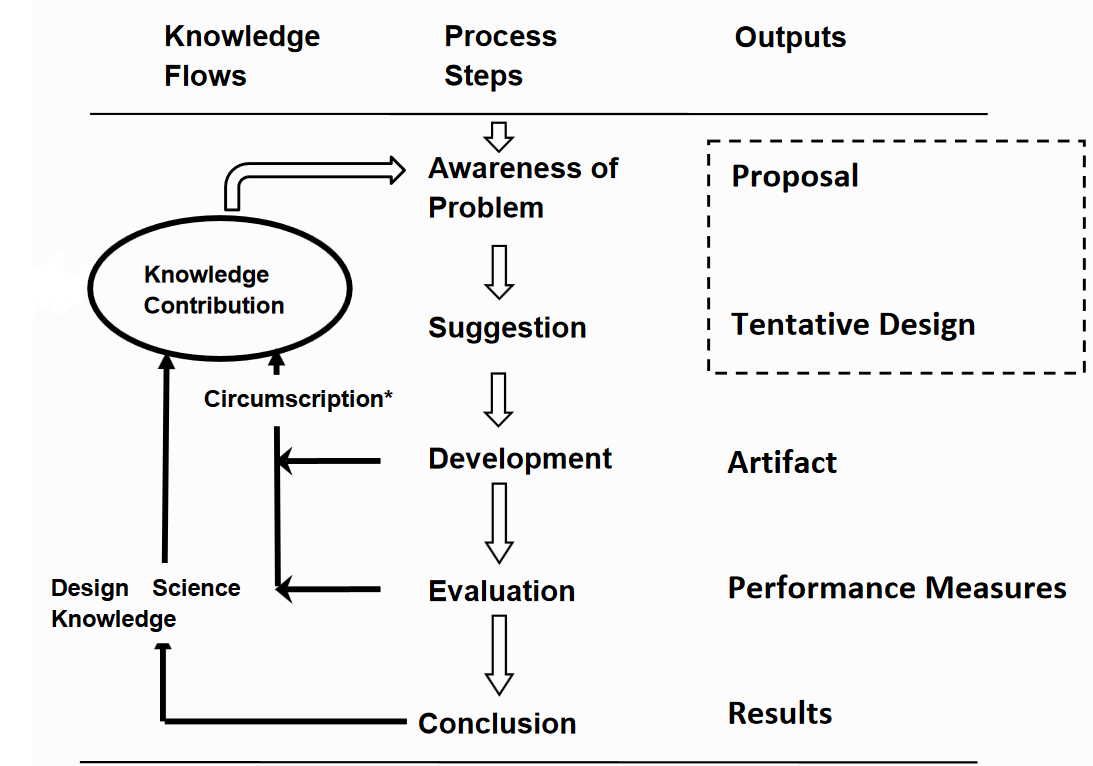
\includegraphics[width=\linewidth]{./res/DSR_Model.png}
 			\caption{Design Science Research Process Model}
 			%http://desrist.org/desrist/content/design-science-research-in-information-systems.pdf
 		\end{figure}
 	
	}
	

	
	\section{\iflanguage{ngerman}{Einschränkungen}{Limitations and Delimitations}}
	The goal of this study is to create an effective and helpful change recommendation tool to aid during the creation of models. We will still aim to keep the tool as broad as possible so that it can be used for other application in which a change history is available.
	
	Although a user interface and plugin for different model creation software are certainly imaginable, we won't try to archive those goals. Instead a command line interface will be implemented.
	
	
	\section{\iflanguage{ngerman}{Signifikanz der Untersuchung}{Significance of the study}}
	The significance of this study lies within its usability and helpfulness. Streamlining the process of model creation aids to increase the quality of software and its design. The ability to bypass mindless repetition during the creation of a model helps the engineer to focus on the important aspects of that model. 
	
	The creation of this study will also help in deepening my knowledge in functional programming and machine learning. Both of which serve as useful tools for any programmer. With the former being an additional paradigm with which to program and the latter being a relevant topic in almost every aspect of computer science.
	
	
	\section{\iflanguage{ngerman}
		{Planung}
		{Planning}}
	\label{sec:planning}
	
	\subsection{\iflanguage{ngerman}
		{Eigene Vorkenntnisse}
		{Own Background}}
	\label{sub:background}
	My knowledge in functional programming, while lean, serves as a good start for the creation of this study. Especially when supported by my background with lectures such as "Programmierung von Systemen" and "Algorithmen und Datenstrukturen" as a student as well as a tutor. Both of which are highly applicable in this study. My participation in "Sopra 16/17" provides me with experience for the designing, implementation and testing of the tool which we aim to create. 
	
	Having said that, extensive practice in practical functional programming will be necessary as well as attaining knowledge in machine learning, especially regression algorithms. My successful completion of the lecture "Einführung in die künstliche Intelligenz" and the proseminar "Algorithmen" will hopefully provide a strong base for that.
	
	\subsection{\iflanguage{ngerman}
		{Benötigte Ressourcen}
		{Required Resources}}
	\label{sub:resources}
	No especial resources will be necessary. Only access to data in form of model histories and the tool SiLift should suffice for the creation of this study.
	
	\subsection{\iflanguage{ngerman}
		{Zeitplanung}
		{Work packages}}
	\label{sub:wp}
	
	\iflanguage{ngerman}
	
	\begin{description}
		\item[M1] Extensive practice in Haskell, especially data-analysis. Research into decision trees and other applicable data-structures.
		\item[M2] Analysis and first design of a solution.
		\item[M3-4] Multiple iterations of deign - implementation - review.
		\item[M5] Final implementation. Testing of tool, comparison with similar tools.
		\item[M6] Collection of results on paper, answering all research questions.
	\end{description}
	
	\subsection{\iflanguage{ngerman}
		{Risiken und Ausweichplan}
		{Contingency plan}}
	\label{sub:contingency}
	
	\iflanguage{ngerman}
	
	\begin{enumerate}
		\item Failing to create such a tool with Haskell due to lacking knowledge. This eventuality will be discussed with the creators of the study.
	\end{enumerate}
	
	\nocite{*}
	\printbibliography
	
\end{document}

